\documentclass[xcolor=dvipsnames]{beamer}  % ALLOWS CHANGE IN COLOR
\usepackage{beamerthemesplit}

%% commenting the above and uncommenting below prints handout (use 4 on 1 or 8 on 1)
% \documentclass[handout,xcolor=dvipsnames]{beamer}     % TO PRINT PRESENTATION HANDOUT
% \usepackage{pgfpages}
% \pgfpagesuselayout{8 on 1}[letter, border shrink=5mm]

\usepackage{url}
\usepackage{ae} % or {zefonts}
\usepackage[T1]{fontenc}
\usepackage[ansinew]{inputenc}
\usepackage[spanish,es-nodecimaldot]{babel}

\usepackage{amsmath}

\usepackage{graphicx}
%\graphicspath{"../../graphs/"}
\usepackage{color}
%\usepackage[colorlinks]{hyperref} % beamer loads this by default, needed only to change default behavior? 
\usepackage{tikz} % Easier syntax to draw pgf files (invokes pgf automatically)
\usetikzlibrary{arrows,shapes.geometric}

\usepackage{tabulary} % automatic column length in tables with long text string
%% use LRJC for auto, and lrjc for normal column width
\setlength\tymin{10pt}       %% change behavior, see p. 254 LaTeX companion
\setlength\tymax{\maxdimen}  %% change behavior, see p. 254 LaTeX companion

\usepackage{multirow} %allows multiple rows in tables

%\usecolortheme{crane}     %Color yellow
%\usetheme{Warsaw}
\usecolortheme[named=Gray]{structure}

\useoutertheme[footline=empty]{}  % PUTS COLORED LINE AT FOOT WITH TITLE, AUTHOR, PAGE, etc
%\usetheme{Berkeley}
\usetheme[height=7mm]{Rochester}
\setbeamertemplate{items}[ball]   % ITEMS IN 3D BALLS (alt CIRCLES)
\setbeamertemplate{navigation symbols}{}  % DROPS NAVIGATION ICONS
\setbeamertemplate{blocks}[rounded][shadow=true]

%\setbeamertemplate{footline} {
%    \begin{beamercolorbox}{section in head/foot}
%    \insertsectionnavigationhorizontal{\paperwidth}{}{plus1filll
%    \insertframenumber}
%    \end{beamercolorbox}
%}

%\setbeamertemplate{navigation symbols}{\insertslidenavigationsymbol,
%\insertdocnavigationsymbol} \setbeamertemplate{footline} {
%    \begin{beamercolorbox}{section in head/foot}
%    \insertsectionnavigationhorizontal{\paperwidth}{}{plus1filll
%    \insertframenumber}
%    \end{beamercolorbox}
%}

\setbeamercovered{transparent}
\setbeamertemplate{caption}{\insertcaption}
\setbeamertemplate{footline}[frame number] % adds slide number, overrides split footer with authors/title that the theme uses

\tikzstyle{nodo} = [circle, draw=black, fill=white, text=black]
\tikzstyle{end} = [circle, minimum width=3pt,fill, inner sep=0pt]

\AtBeginSection[] {
   \begin{frame}
       \frametitle{Road map}
       \tableofcontents[currentsection]
   \end{frame}
}

\title[Malapportionment \& bias]{Malapportionment, party bias and responsiveness in Mexico's mixed-member system}
%\subtitle{Party bias and responsiveness in Mexico}
\author[Magar, Trelles, Altman, McDonald]{E. Magar\inst{1}  \and A. Trelles\inst{2} \and M. Altman\inst{3} \and M.P. McDonald\inst{4}}
\institute[ITAM-MIT-UFG-Pitt]{\inst{1} ITAM \and 
                              \inst{2} University of Pittsburgh \and
                              \inst{3} MIT \and
                              \inst{4} UF, Gainesville}
%\address{}
\date[13mar15]{University of Florida, Gainesville \\ 3/13/15}

\begin{document}

%%%%%%%%%%%%%%%%%%%%%%%%%%%%%%%%%%%%%%%%%%%%%%%%%%%%%%%%%%%%%%%%%%%%%%%%%%%%%%%%%%%%%%%%%%%%

\frame[plain]{\titlepage}

%%%%%%%%%%%%%%%%%%%%%%%%%%%%%%%%%%%%%%%%%%%%%%%%%%%%%%%%%%%%%%%%%%%%%%%%%%%%%%%%%%%%%%%%%%%%
\begin{frame}                      % SLIDE

    \frametitle{Motivation}

How does redistricting affect representation?

\begin{itemize}
\item Taking map drawing out of the hands of politicians \\ does not necessarily ensure a fair result
\end{itemize}

\bigskip

Does malapportionment introduce political bias?

\begin{itemize}
\item Sparsely populated areas get same representation as the densely populated
\end{itemize}

\bigskip

\pause

\begin{block}{How does Mexico fare?}

\begin{enumerate}
\item Malapportionment is substantial
\item Political distorsions? 
  \begin{itemize}
  \item Not much party bias
  \item but big large-party bonus
  \item party sensitivities to boundary changes differ a lot
  \end{itemize}
\end{enumerate}

\end{block}

\end{frame}
%%%%%%%%%%%%%%%%%%%%%%%%%%%%%%%%%%%%%%%%%%%%%%%%%%%%%%%%%%%%%%%%%%%%%%%%%%%%%%%%%%%%%%%%%%%%%%%%
\frame {                      % SLIDE
    \frametitle{Road map}
\tableofcontents%[section=1]
}
%%%%%%%%%%%%%%%%%%%%%%%%%%%%%%%%%%%%%%%%%%%%%%%%%%%%%%%%%%%%%%%%%%%%%%%%%%%%%%%%%%%%%%%%%%%%%%%%
\section{Malapportionment}
%%%%%%%%%%%%%%%%%%%%%%%%%%%%%%%%%%%%%%%%%%%%%%%%%%%%%%%%%%%%%%%%%%%%%%%%%%%%%%%%%%%%%%%%%%%% 
\begin{frame}                      % SLIDE

    \frametitle{Comparative perspective}


UK and US

\begin{itemize}
\item instills bias when one party strong in small districts \\ (as Tories were up to 1997, Johnston 2002)
\item Reapportionment Revolution removed bias in \\ different, predictable degrees (Cox\&Katz 2002)
\item no party bias from malapp.\ after mid-1960s \\ (Grofman et al.~1997)
\end{itemize}

\end{frame}

%%%%%%%%%%%%%%%%%%%%%%%%%%%%%%%%%%%%%%%%%%%%%%%%%%%%%%%%%%%%%%%%%%%%%%%%%%%%%%%%%%%%%%%%%%%% 
\begin{frame}                      % SLIDE

    \frametitle{Worldwide description}

Samuels\&Snyder (2001): mean absolute district deviation from ideal size in 78 countries 

\bigskip

\begin{footnotesize}
\begin{tabular}{rlrr}
Rank & case & MAL & Year \\ \hline
1 & Tanzania & 0.262 & 1995 \\
2 & Korea & 0.208 & 1996 \\
3 & Ecuador & 0.204 & 1998 \\
4 & Kenya & 0.195 & 1997 \\
5 & Ghana & 0.178 & 1996 \\
11 & Chile & 0.151 & 1997 \\
12 & Argentina & 0.141 & 1995 \\
14 & Colombia & 0.132 & 1994 \\
16 & Spain & 0.096 & 1996 \\
17 & Brazil & 0.091 & 1998 \\
31 & \alert{Mexico} & 0.064 & 1997 \\
40 & UK & 0.046 & 1997 \\
64 & US & 0.014 & 1992 \\
78 & Israel & 0.000 & 1999 \\
\end{tabular}
\end{footnotesize}

\end{frame}
%%%%%%%%%%%%%%%%%%%%%%%%%%%%%%%%%%%%%%%%%%%%%%%%%%%%%%%%%%%%%%%%%%%%%%%%%%%%%%%%%%%%%%%%%%%% 
\begin{frame}                      % SLIDE

    \frametitle{Some sources of malapportionment}

Malapportionment can be intentional or not

\bigskip

\begin{tabular}{cll}
   & Source & Intentional? \\ \hline
(1)& relative population shifts &no \\
(2)& apportionment of seats to states &no \\
(3)& optimization rules &? \\
(4)& use of old population estimates &? \\
(5)& gerrymandering &yes \\\hline
\end{tabular}

\bigskip

Some findings:

\begin{itemize}
\item (4) affects (2) and (3)
\item Redistricting affects parties quite differently \\ (PAN most sensitive, PRI least)
\end{itemize}

\end{frame}
%%%%%%%%%%%%%%%%%%%%%%%%%%%%%%%%%%%%%%%%%%%%%%%%%%%%%%%%%%%%%%%%%%%%%%%%%%%%%%%%%%%%%%%%%%%%%%%%
\section{Redistricting in Mexico}
%%%%%%%%%%%%%%%%%%%%%%%%%%%%%%%%%%%%%%%%%%%%%%%%%%%%%%%%%%%%%%%%%%%%%%%%%%%%%%%%%%%%%%%%%%%%%%%%
\begin{frame}                      % SLIDE

    \frametitle{Background on Mexico}

\begin{itemize}

\item 32 states, 2.5k municipalities, 67k electoral \emph{secciones}

\item Hegemonic party 1929--2000 

\item Lower chamber of Congress elected every 3 years

  \begin{itemize}

  \item SMD only until 1961
  \item Mixed system since 1979: 300 SMD + 200 PR seats

  \end{itemize}
  
\item Single-term limits removed in 2018

\item Autonomous EMB (IFE, now INE) organizes elections and redistricting

\end{itemize}

\end{frame}
%%%%%%%%%%%%%%%%%%%%%%%%%%%%%%%%%%%%%%%%%%%%%%%%%%%%%%%%%%%%%%%%%%%%%%%%%%%%%%%%%%%%%%%%%%%% 

\begin{frame}                      % SLIDE
    \frametitle{The redistricting process}
\begin{center}
   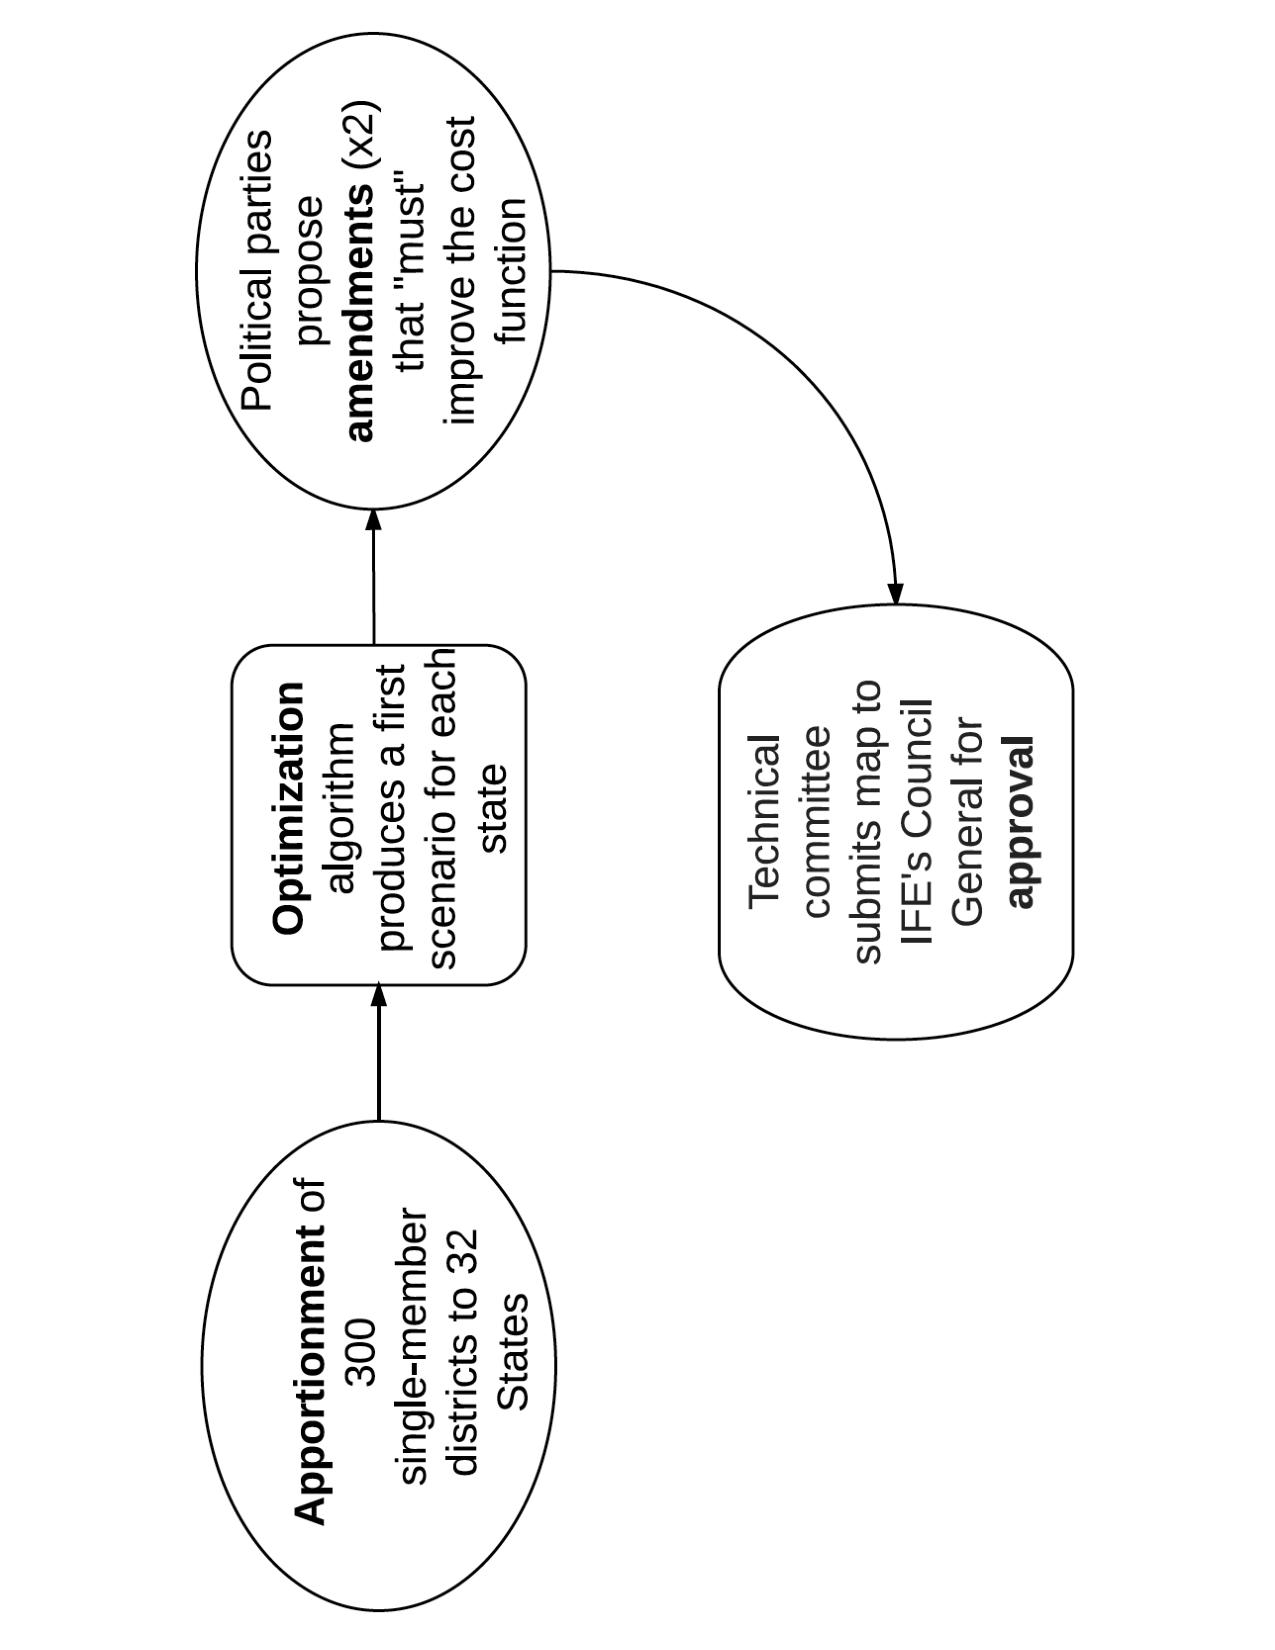
\includegraphics[width=8cm, angle=-90]{../../graphs/mexRedisProcessFlowchart.pdf}
\end{center}

\end{frame}
%%%%%%%%%%%%%%%%%%%%%%%%%%%%%%%%%%%%%%%%%%%%%%%%%%%%%%%%%%%%%%%%%%%%%%%%%%%%%%%%%%%%%%%%%%%% 
\begin{frame}                      % SLIDE
    \frametitle{Apportionment}


Hamilton method used:

\begin{itemize}
\item The quota (or price of a seat) is $Q = \frac{\text{nation's population}}{300}$

\item First allocation is $\frac{\text{state's population}}{Q}$, rounded down

\item Every state gets 2 seats min

\item Unallocated seats, if any, awarded to states with largest fractional remainders
\end{itemize}

\bigskip

\pause

Most recent decennial census must be used 

\begin{itemize}
\item ... but no obligation to redistrict as soon as available
\item 6-year lag on average: 199\textbf{7}, 200\textbf{6}, 201\textbf{5}
%\item and IFE considers $\pm15\%$ imbalance normal (!)
\end{itemize}

\end{frame}
%%%%%%%%%%%%%%%%%%%%%%%%%%%%%%%%%%%%%%%%%%%%%%%%%%%%%%%%%%%%%%%%%%%%%%%%%%%%%%%%%%%%%%%%%%%% 

\begin{frame}                      % SLIDE

    \frametitle{The redistricting process}

Redistricting by experts in 1997, 2006, 2015 (abandoned), and now 2018

\begin{enumerate}
\item apportionment of 300 seats to 32 states
\item optimization algorithm $\rightarrow$ proposal
\item parties propose amendments (``must'' improve score)
%\item repeat 2 and 3
\item new map
\end{enumerate}

\begin{multline*}
\texttt{Score} = .4 \times \texttt{PopBalance} + .3 \times \texttt{MunicBoundaries} \\
+ .2 \times \texttt{TravelTime} + .1 \times \texttt{Compactness}
\end{multline*}

%\pause

IFE considers $\pm15\%$ imbalance normal (!)


%Salience should go up: single-term limits dropped in 2018

\end{frame}
%%%%%%%%%%%%%%%%%%%%%%%%%%%%%%%%%%%%%%%%%%%%%%%%%%%%%%%%%%%%%%%%%%%%%%%%%%%%%%%%%%%%%%%%%%%% 

\begin{frame}                      % SLIDE
    \frametitle{Optimization algorithm}

Simulated annealing = probabilistic meta-heuristic for optimization \\ locates a good approximation to the global optimum of the cost function in a large search space

\bigskip

Thousands of iterations using electoral \emph{secciones} 

\bigskip

Combinatorial optimization algorithm used to generate 
the first scenario in each state


\begin{center}
   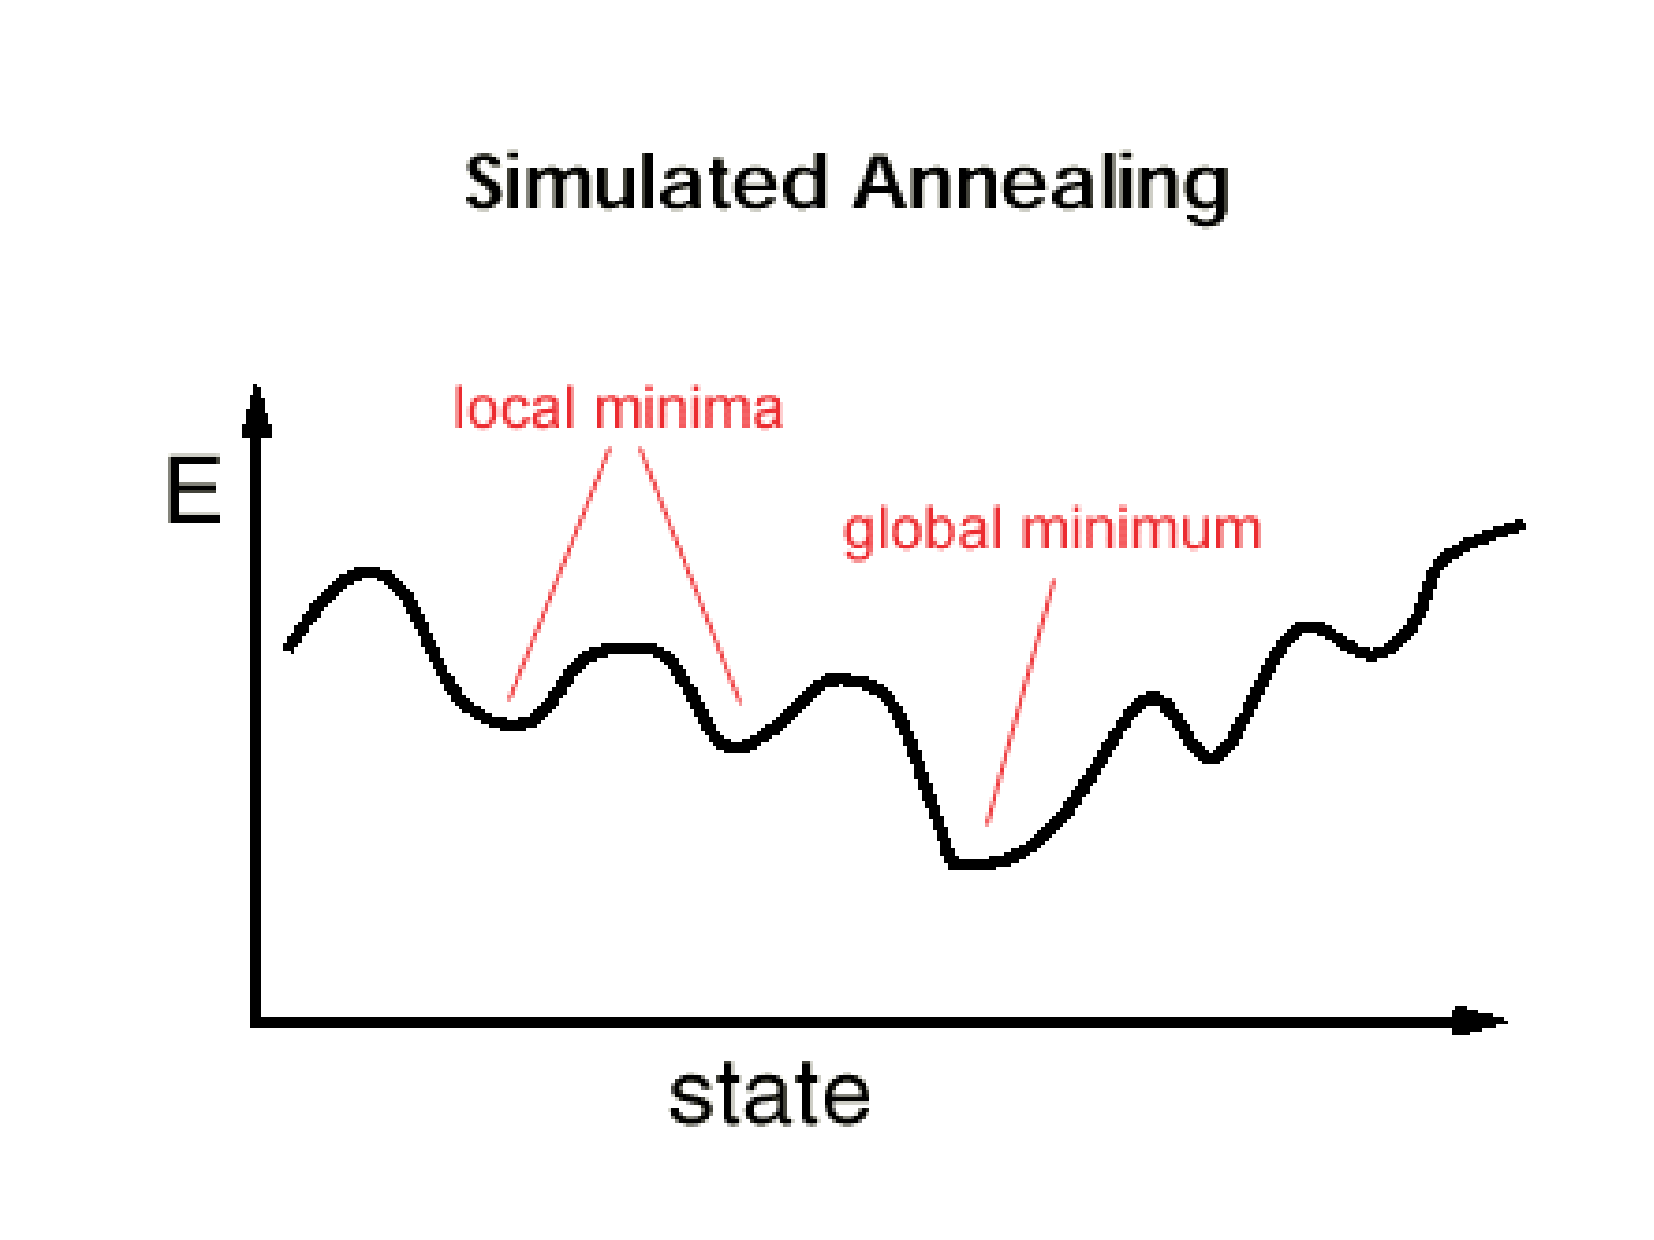
\includegraphics[width=5cm]{../../graphs/sim.pdf}
\end{center}

EMB claims that this is a public process, but the \\ operation and procedures are done \alert{behind closed doors}

\end{frame}
%%%%%%%%%%%%%%%%%%%%%%%%%%%%%%%%%%%%%%%%%%%%%%%%%%%%%%%%%%%%%%%%%%%%%%%%%%%%%%%%%%%%%%%%%%%% 
\begin{frame}                                       % SLIDE

    \frametitle{Party amendments}
\begin{center}
   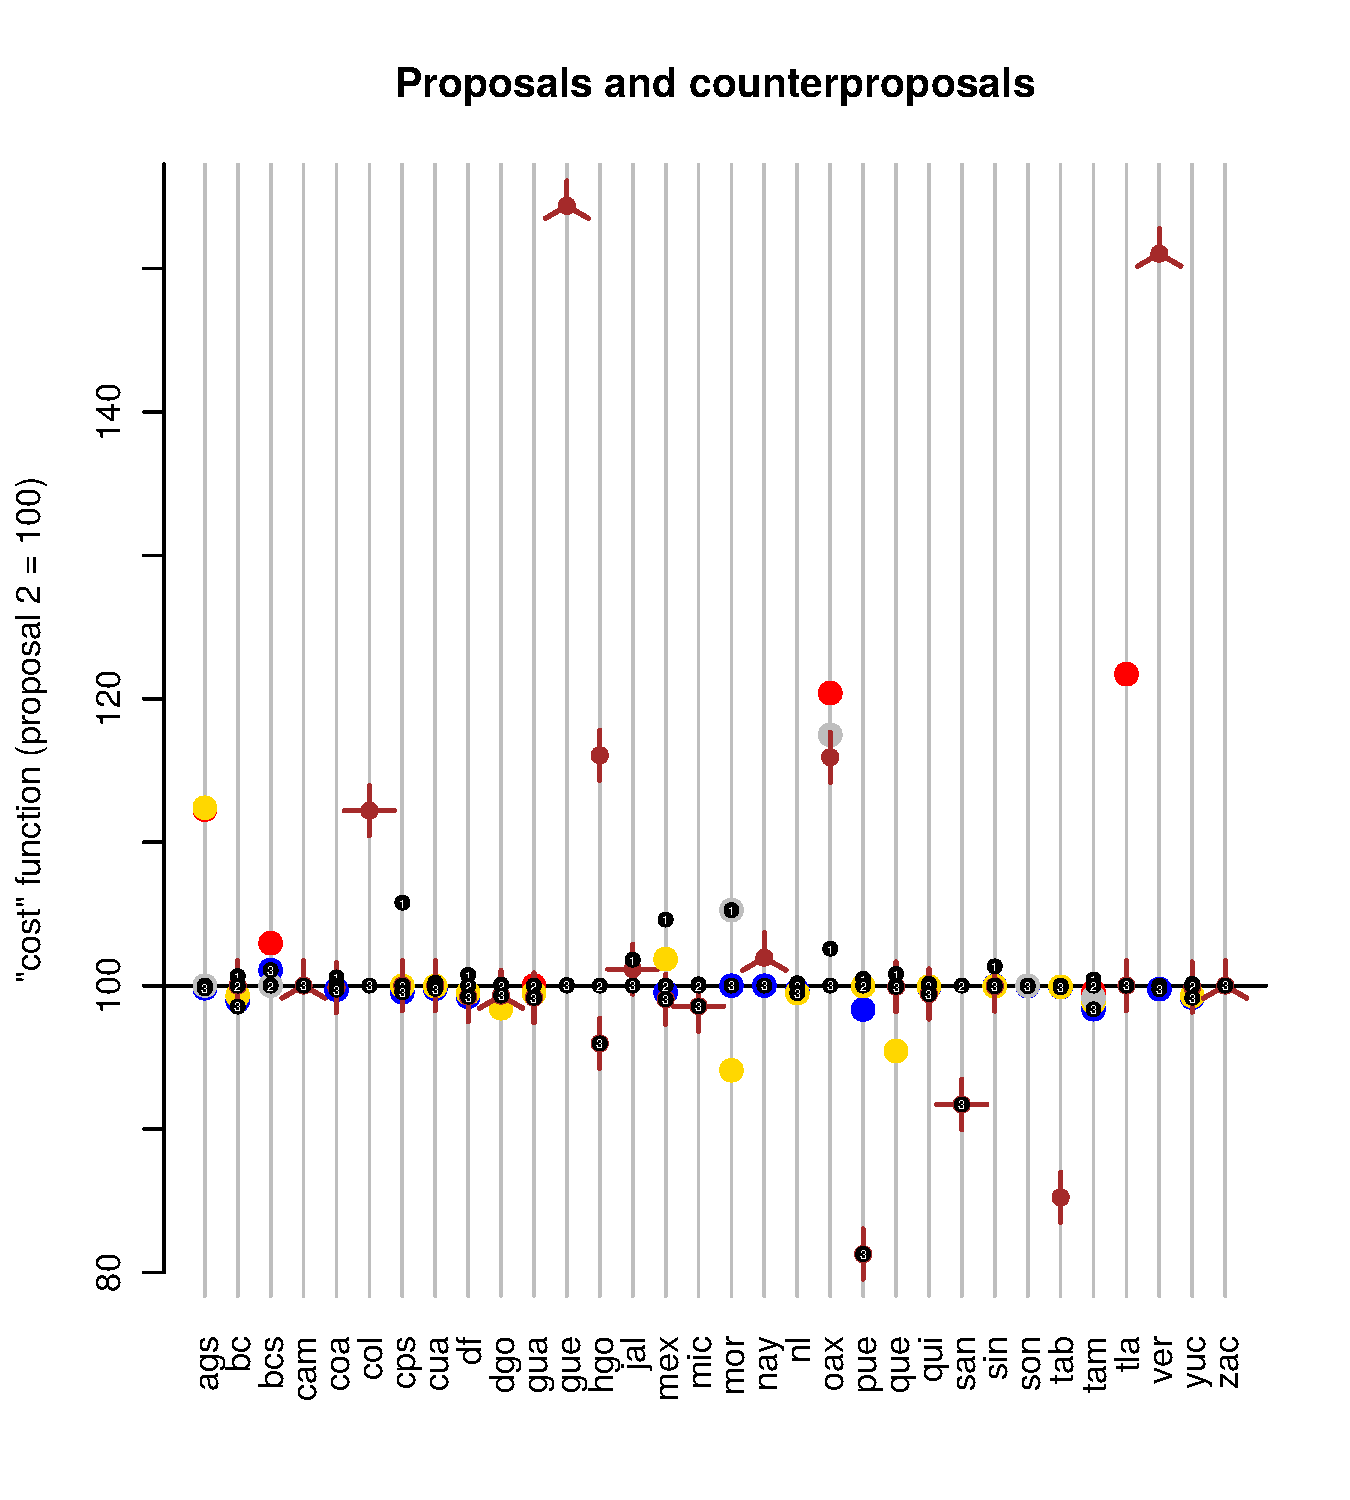
\includegraphics[width=8cm]{../../graphs/propsAndCost.pdf}
\end{center}
\end{frame}
%%%%%%%%%%%%%%%%%%%%%%%%%%%%%%%%%%%%%%%%%%%%%%%%%%%%%%%%%%%%%%%%%%%%%%%%%%%%%%%%%%%%%%%%%%%% 
\begin{frame}                                       % SLIDE

    \frametitle{Party amendments}
\begin{itemize}
\item Humans can beat the computer $\rightarrow$ enables manipulation 
\item Smoking gun: four maps improved score but \alert{not} adopted
\item Unobserved: maps improving score but hurting parties?
\item Increased similarity of final map to status quo: parties protecting strongholds?
\item Asymmetric party capacity to produce counterproposals: by far, PAN most effective. Benefits?
\item Party learning process 
\end{itemize} 

\end{frame}
%%%%%%%%%%%%%%%%%%%%%%%%%%%%%%%%%%%%%%%%%%%%%%%%%%%%%%%%%%%%%%%%%%%%%%%%%%%%%%%%%%%%%%%%%%%% 
\begin{frame}\label{fr:MxMapProj}                      % SLIDE

    \frametitle{The bigger project}

\emph{Draw Mexico} project = offspring of \emph{Public Mapping Project in U.S.}

\bigskip

Remove opaqueness from redistricting process 

\bigskip

\texttt{DistrictBuilder} is open-source, web-based software %({\footnotesize \url{www.districtbuilder.org}}):

\begin{itemize}

\item enables widespread DIY redistricting thru cloud computing

\item  internet lets anyone draw/inspect maps: crowdsourcing

\item redistricting contests in 6 US states $\rightarrow$ hundreds of legal plans

\end{itemize}

\bigskip

Application to \alert{Mexico} \href{http://23.21.151.172/}{\beamergotobutton{Link: MexDemo}} (Donations anyone?) 

\end{frame}
%%%%%%%%%%%%%%%%%%%%%%%%%%%%%%%%%%%%%%%%%%%%%%%%%%%%%%%%%%%%%%%%%%%%%%%%%%%%%%%%%%%%%%%%%%%% 
\section{Data}
%%%%%%%%%%%%%%%%%%%%%%%%%%%%%%%%%%%%%%%%%%%%%%%%%%%%%%%%%%%%%%%%%%%%%%%%%%%%%%%%%%%%%%%%%%%% 
\begin{frame}
    \frametitle{Expectations}
\begin{itemize}
\item Countryside has lost size relative to cities for decades
\item PRI's bases of support (Ames 1970, Moreno 2003): 
  \begin{itemize}
  \item rural 
  \item less educated
  \item less better-off
  \item older
  \end{itemize}
\end{itemize}

\bigskip \pause

\begin{block}{Hypotheses:} 
\begin{enumerate}
\item Does malapportionment introduce PRI-favoring bias?
\item If so, against PAN? PRD? both?
\item Does redistricting remove/reduce bias?
\end{enumerate}
\end{block}

\end{frame}
%%%%%%%%%%%%%%%%%%%%%%%%%%%%%%%%%%%%%%%%%%%%%%%%%%%%%%%%%%%%%%%%%%%%%%%%%%%%%%%%%%%%%%%%%%%% 
\frame {                      % SLIDE
    \frametitle{Votes and SMD seats 2006, 2009, 2012}

State-level aggregates (average = 9.4 districts, larger N) 
%\item 2006--2012 districts constant
%\item MCMC \footnotesize{($3 \times 10k$ iter., every $100^{th}$ for post.\ sample)}

 \begin{columns}[c]

 \column{.8\textwidth}

\begin{center}
   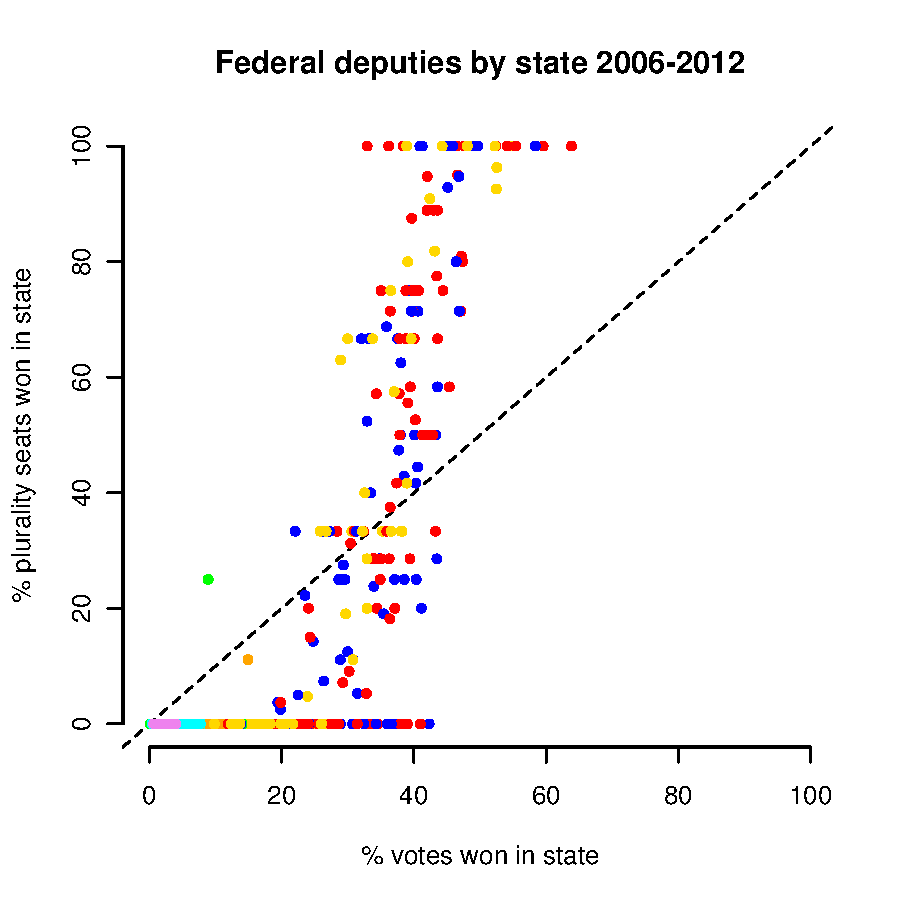
\includegraphics[width=6cm]{../../graphs/resXedo20062012.pdf}
\end{center}

 \column{.2\textwidth}

{\color{blue} PAN} \\ {\color{red} PRI} \\ {\color{yellow} PRD} \\ {\color{green} Green}

\end{columns}

\begin{tabular}{rr}
State-years above 45� line:~~PRI & $^3/_5$ \\
PAN & $^2/_5$ \\
PRD & $^1/_4$ \\
\end{tabular}

}
%%%%%%%%%%%%%%%%%%%%%%%%%%%%%%%%%%%%%%%%%%%%%%%%%%%%%%%%%%%%%%%%%%%%%%%%%%%%%%%%%%%%%%%%%%%% 

\begin{frame}                      % SLIDE
    \frametitle{States' representation}

\begin{center}
   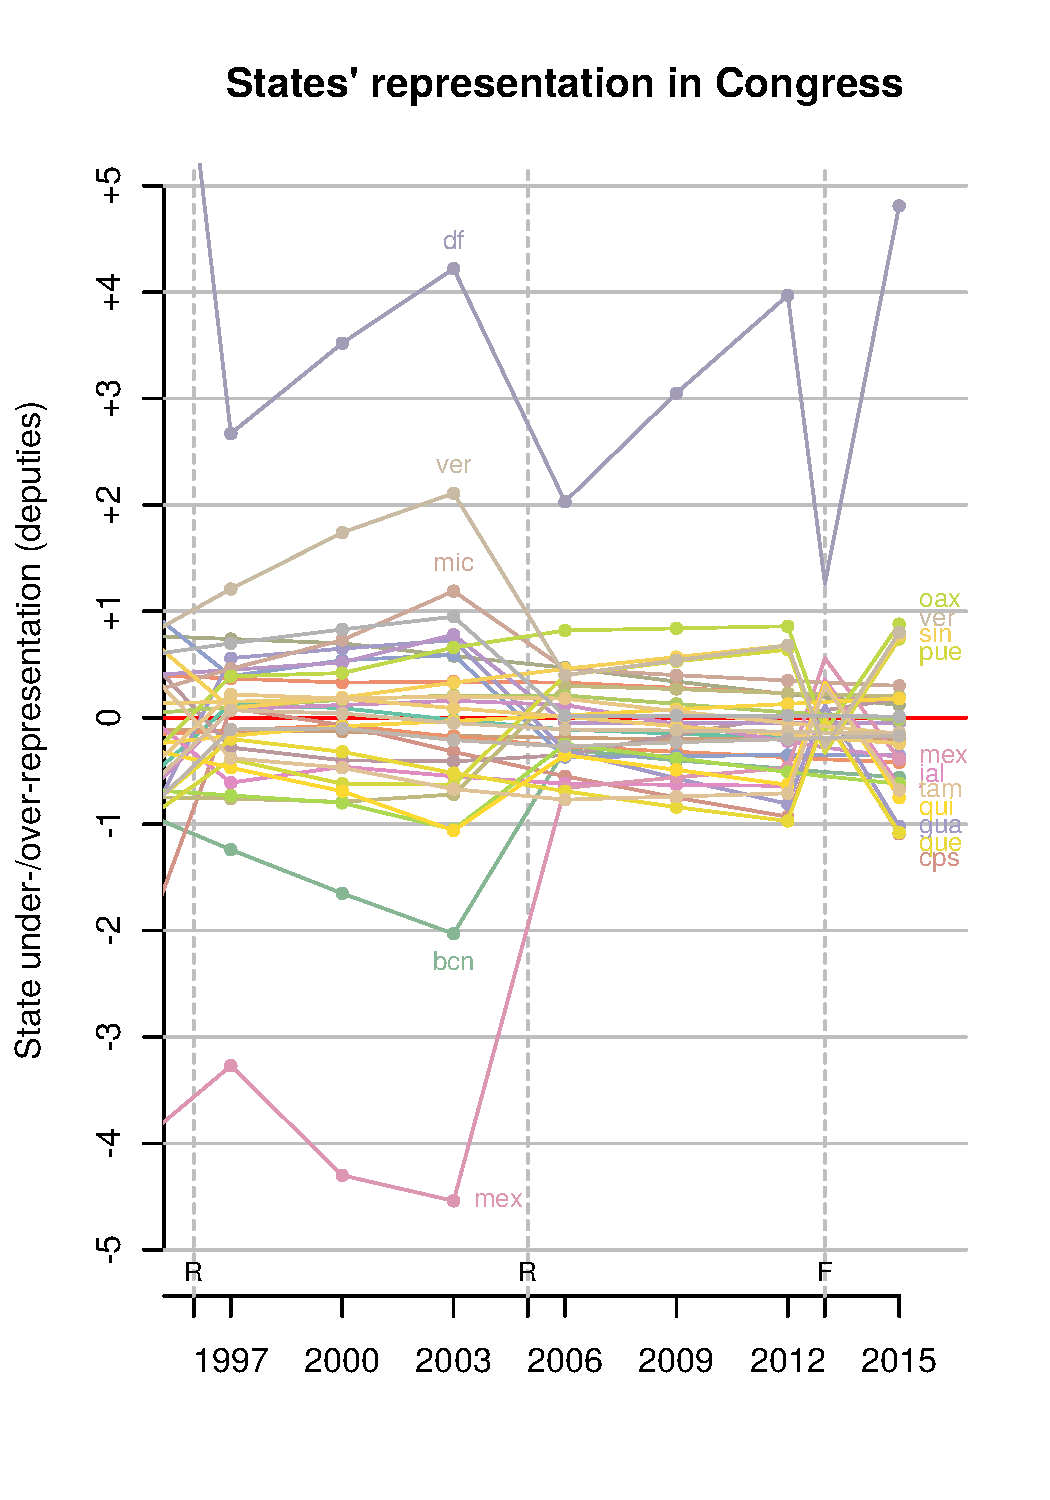
\includegraphics[width=6cm]{../../graphs/statesUnderOverRep.pdf}
\end{center}

\end{frame}
%%%%%%%%%%%%%%%%%%%%%%%%%%%%%%%%%%%%%%%%%%%%%%%%%%%%%%%%%%%%%%%%%%%%%%%%%%%%%%%%%%%%%%%%%%%% 

\frame {                      % SLIDE
    \frametitle{States' representation}

\begin{center}
   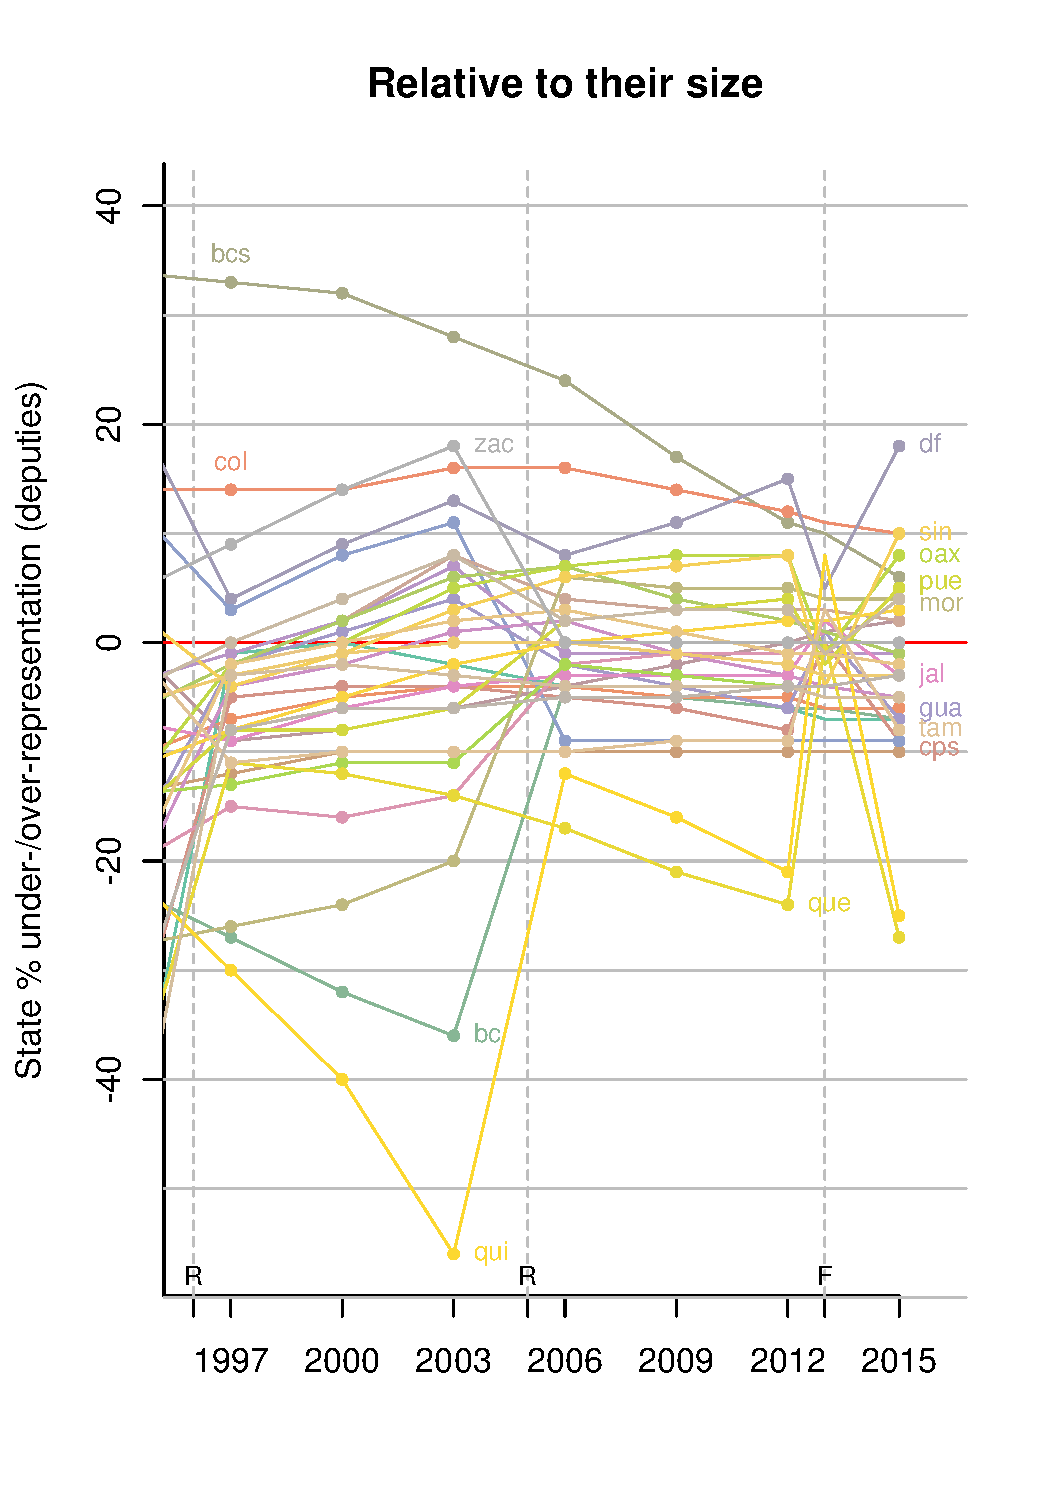
\includegraphics[width=6cm]{../../graphs/statesUnderOverRep-rel.pdf}
\end{center}

}
%%%%%%%%%%%%%%%%%%%%%%%%%%%%%%%%%%%%%%%%%%%%%%%%%%%%%%%%%%%%%%%%%%%%%%%%%%%%%%%%%%%%%%%%%%%% 
\frame {                      % SLIDE
    \frametitle{States' representation}

Use of population projections reveals unintended malapportionment \\

\bigskip

And use of old population estimates introduces distorsions

\bigskip

Relative representation index (Ansolabehere et al. 2002):

\bigskip

$RRI_{d,s} = \frac{1/population_d}{apportionment_s/population_s}$

\bigskip 

(Reformers should demand use of fresher population estimates!)
}
%%%%%%%%%%%%%%%%%%%%%%%%%%%%%%%%%%%%%%%%%%%%%%%%%%%%%%%%%%%%%%%%%%%%%%%%%%%%%%%%%%%%%%%%%%%% 

\frame {                      % SLIDE
    \frametitle{Representation within states}

\begin{center}
   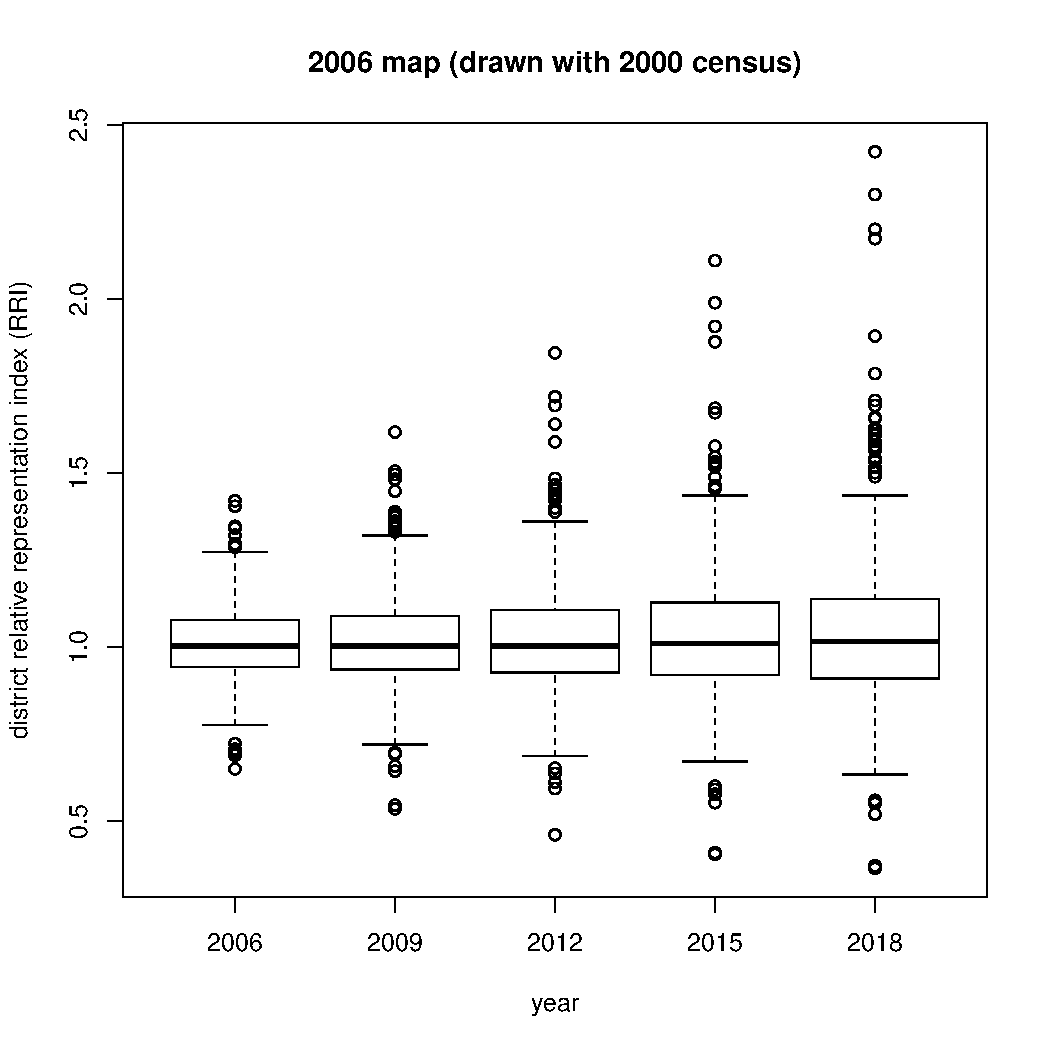
\includegraphics[width=.75\columnwidth]{../../graphs/rris0618d0.pdf} 
\end{center}

}
%%%%%%%%%%%%%%%%%%%%%%%%%%%%%%%%%%%%%%%%%%%%%%%%%%%%%%%%%%%%%%%%%%%%%%%%%%%%%%%%%%%%%%%%%%%% 

\frame {                      % SLIDE
    \frametitle{Representation within states}

\begin{center}
   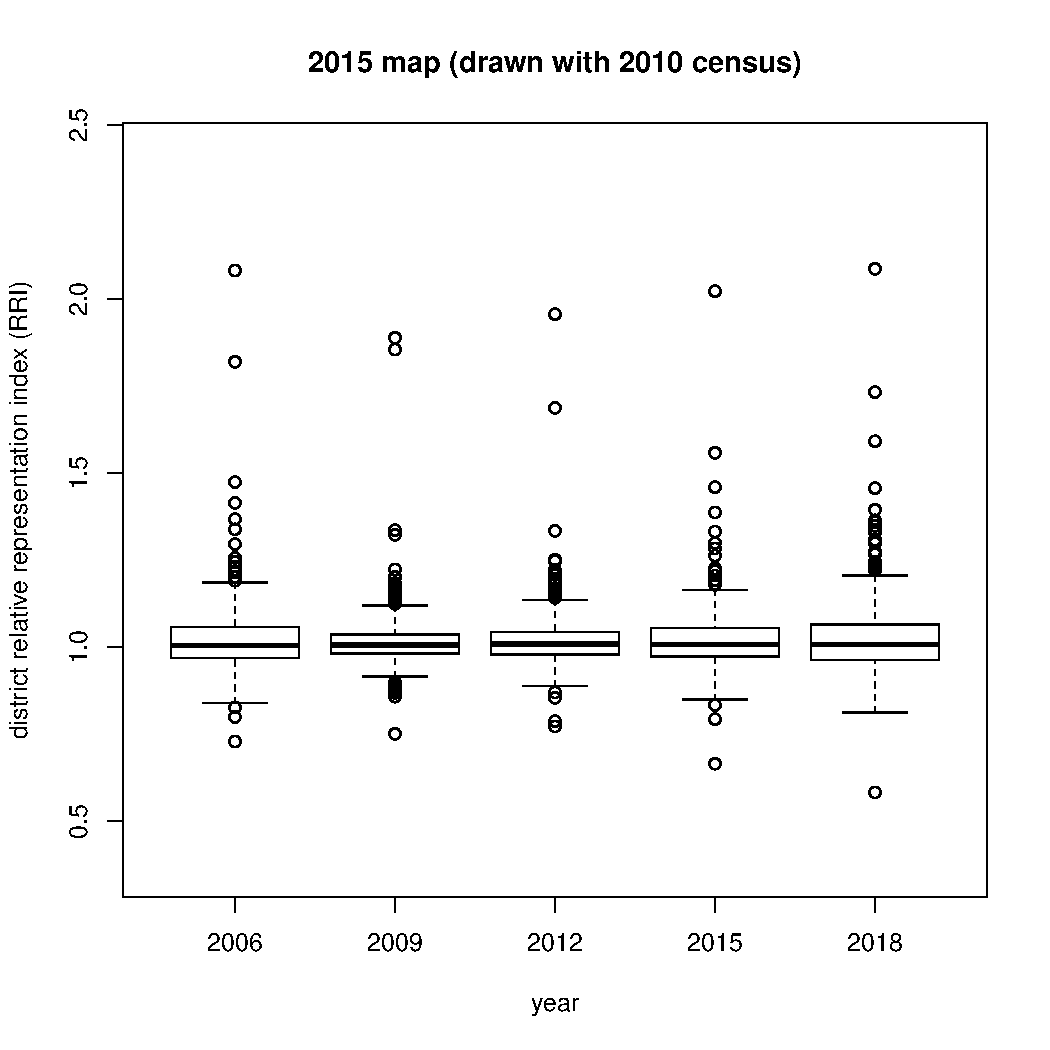
\includegraphics[width=.75\columnwidth]{../../graphs/rris0618d3.pdf}
\end{center}

}
%%%%%%%%%%%%%%%%%%%%%%%%%%%%%%%%%%%%%%%%%%%%%%%%%%%%%%%%%%%%%%%%%%%%%%%%%%%%%%%%%%%%%%%%%%%% 
\section{Results: party bias, responsiveness, swing ratios}
%%%%%%%%%%%%%%%%%%%%%%%%%%%%%%%%%%%%%%%%%%%%%%%%%%%%%%%%%%%%%%%%%%%%%%%%%%%%%%%%%%%%%%%%%%%% 

\frame {                      % SLIDE

    \frametitle{Systemic distorsion: two types}

Focus in the \alert{votes-to-seats} relation \\ (Rae 1967, Tufte 1973, Lijphart 1994, Taagepera\&Shugart 1989)

\bigskip

Two measures of interest:

\begin{enumerate}

\item \textbf{Party bias} $\lambda$: \\ helps beneficiary buy seats with fewer votes \\ (``packing'')

\item \textbf{Responsiveness} $\rho$: \\ seat bonus to large parties \\ (``microcosm strategy'')

\end{enumerate}

}

%%%%%%%%%%%%%%%%%%%%%%%%%%%%%%%%%%%%%%%%%%%%%%%%%%%%%%%%%%%%%%%%%%%%%%%%%%%%%%%%%%%%%%%%%%%% 

\frame {                      % SLIDE

    \frametitle{Two types of distorsion}

\begin{center}
   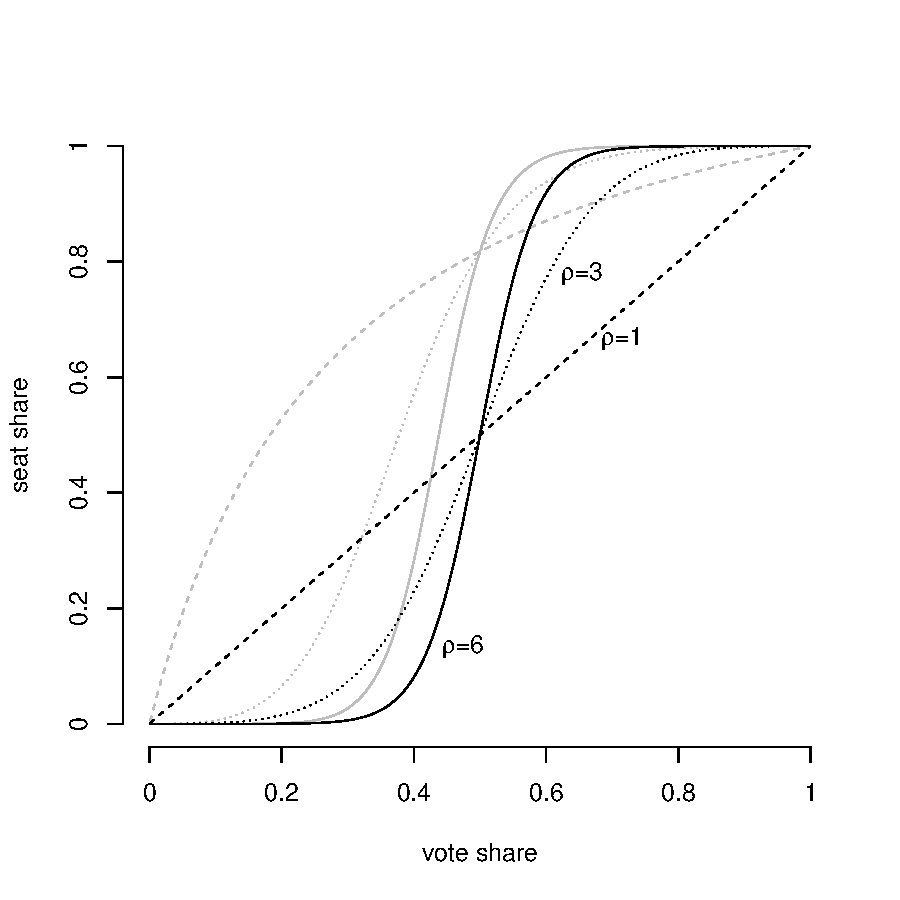
\includegraphics[width=8cm]{../../graphs/rhoExample.pdf}
\end{center}

}
%%%%%%%%%%%%%%%%%%%%%%%%%%%%%%%%%%%%%%%%%%%%%%%%%%%%%%%%%%%%%%%%%%%%%%%%%%%%%%%%%%%%%%%%%%%% 

\frame {                      % SLIDE

    \frametitle{Formalization}

Cube Law:  \begin{equation*}  \frac{s}{1-s} = \left(\frac{v}{1-v}\right)^3 \end{equation*} 

\bigskip

Generalization (King\&Browning 1987):
\begin{equation*}
 \frac{s}{1-s} = e^\lambda *  \left(\frac{v}{1-v}\right)^\rho %\iff  \texttt{logit}(s) = \lambda + \rho *  \texttt{logit}(v)
\end{equation*}

\bigskip

Multiparty (King 1990, Calvo\&Micozzi 2005):
\begin{equation*}
 E(s_j) = \frac{e^{\lambda_j} * v_j^\rho}{\sum_{m=1}^{J} e^{\lambda_m} * v_m^\rho}
\end{equation*}


}

%%%%%%%%%%%%%%%%%%%%%%%%%%%%%%%%%%%%%%%%%%%%%%%%%%%%%%%%%%%%%%%%%%%%%%%%%%%%%%%%%%%%%%%%%%%% 

\frame {                      % SLIDE
    \frametitle{Data}

 \begin{columns}[c]

 \column{.8\textwidth}

\begin{center}
   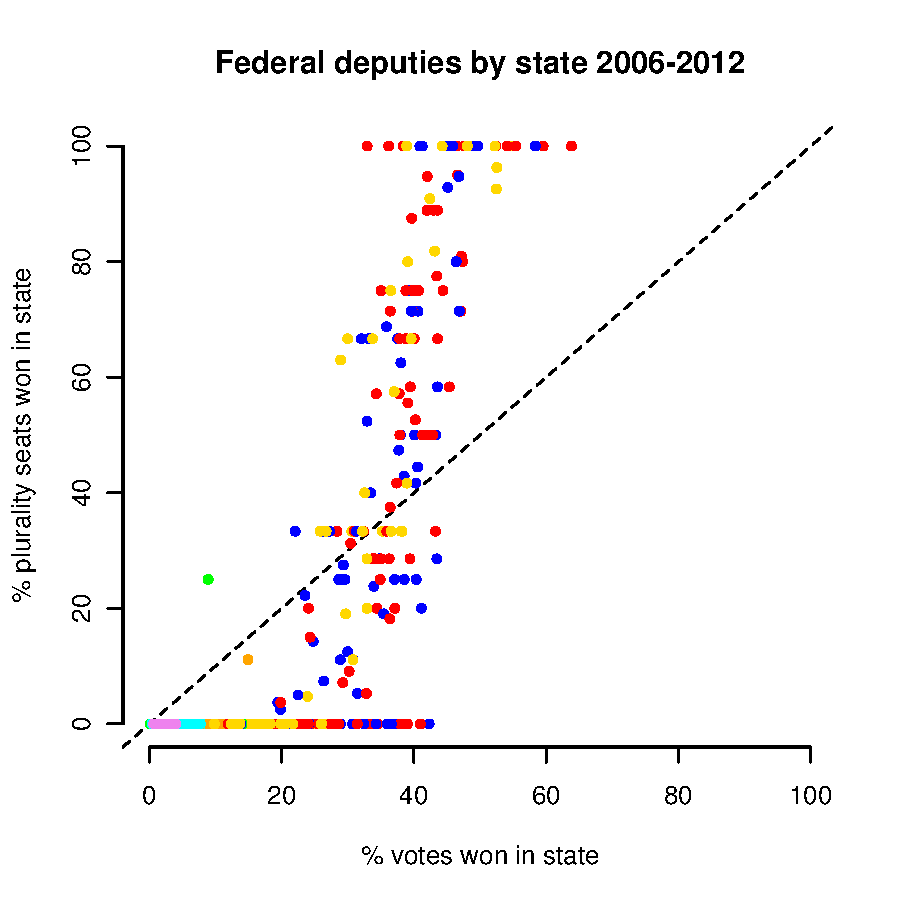
\includegraphics[width=6cm]{../../graphs/resXedo20062012.pdf}
\end{center}

 \column{.2\textwidth}

{\color{blue} PAN} \\ {\color{red} PRI} \\ {\color{yellow} PRD} \\ {\color{green} Green}

\end{columns}

\begin{itemize}
\item State-level aggregates (average = 9.4 districts)
%\item 2006--2012 districts constant
\item MCMC \footnotesize{($3 \times 10k$ iter., every $100^{th}$ for post.\ sample)}
\end{itemize}
}
%%%%%%%%%%%%%%%%%%%%%%%%%%%%%%%%%%%%%%%%%%%%%%%%%%%%%%%%%%%%%%%%%%%%%%%%%%%%%%%%%%%%%%%%%%%% 

\begin{frame}[fragile=singleslide]\frametitle{Bugs code}
\begin{tiny}
\begin{verbatim}
    for (i in 1:I){     # loop over state-years
        for (j in 1:J){ # loop over parties (dummy selects those who ran that year) 
            S[i,j] ~ dbin(pi[i,j], D[i])  # D is number SMD seats in obs. i's state
        }
        numerator[i,1] <- dummy[i,1] * exp( lambda[1] + rho * log(v[i,1]) )
        numerator[i,2] <- dummy[i,2] * exp(             rho * log(v[i,2]) )
        for (j in 3:J){
            numerator[i,j] <- dummy[i,j] * exp( lambda[j-1] ) * v[i,j]^rho
        }
        for (j in 1:J){ # loop over parties (dummy selects those who ran that year) 
            d1[i,j] <- dummy[i,1] * exp( lambda[1] ) * v[i,1]^rho 
            d2[i,j] <- dummy[i,2]                    * v[i,2]^rho 
            d3[i,j] <- dummy[i,3] * exp( lambda[2] ) * v[i,3]^rho 
            d4[i,j] <- dummy[i,4] * exp( lambda[3] ) * v[i,4]^rho 
            d5[i,j] <- dummy[i,5] * exp( lambda[4] ) * v[i,5]^rho 
            d6[i,j] <- dummy[i,6] * exp( lambda[5] ) * v[i,6]^rho 
            d7[i,j] <- dummy[i,7] * exp( lambda[6] ) * v[i,7]^rho 
            denominator[i,j] <- d1[i,j]+d2[i,j]+d3[i,j]+d4[i,j]+d5[i,j]+d6[i,j]+d7[i,j]
            pi[i,j] <- numerator[i,j] / denominator[i,j]
        }
    }
    ### priors
    for (p in 1:6){ # there are 7 party labels in the 3-election data, PRI is reference
        lambda[p] ~ dnorm( 0, tau.lambda )
    }
    tau.lambda <- pow(.25, -2)
    rho ~ dexp(.75) # this has positive range, median close to 1, mean 1.25, max 4.5
\end{verbatim}
\end{tiny}

\end{frame}

%%%%%%%%%%%%%%%%%%%%%%%%%%%%%%%%%%%%%%%%%%%%%%%%%%%%%%%%%%%%%%%%%%%%%%%%%%%%%%%%%%%%%%%%%%%% 

\frame {                      % SLIDE
    \frametitle{Results: party bias relative to PRI}
\begin{center}
\begin{tabular}{cc}
   2006 map & 2015 map \\
   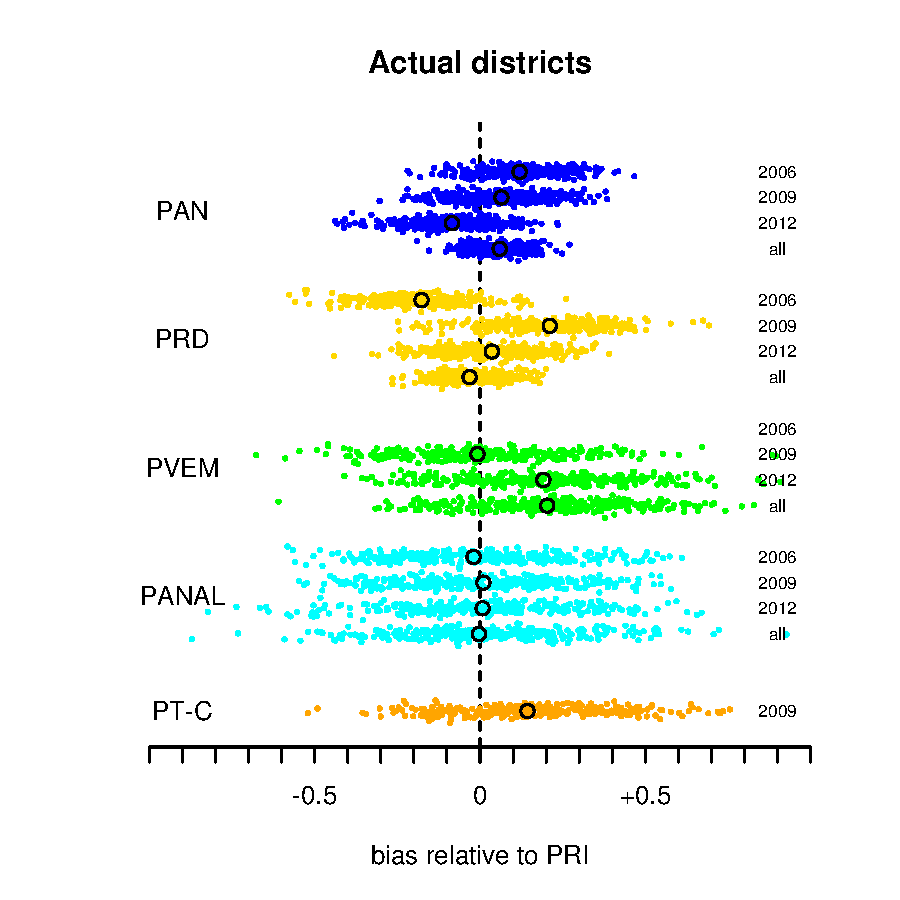
\includegraphics[width=5cm]{../../graphs/bias200612s0.pdf} &
   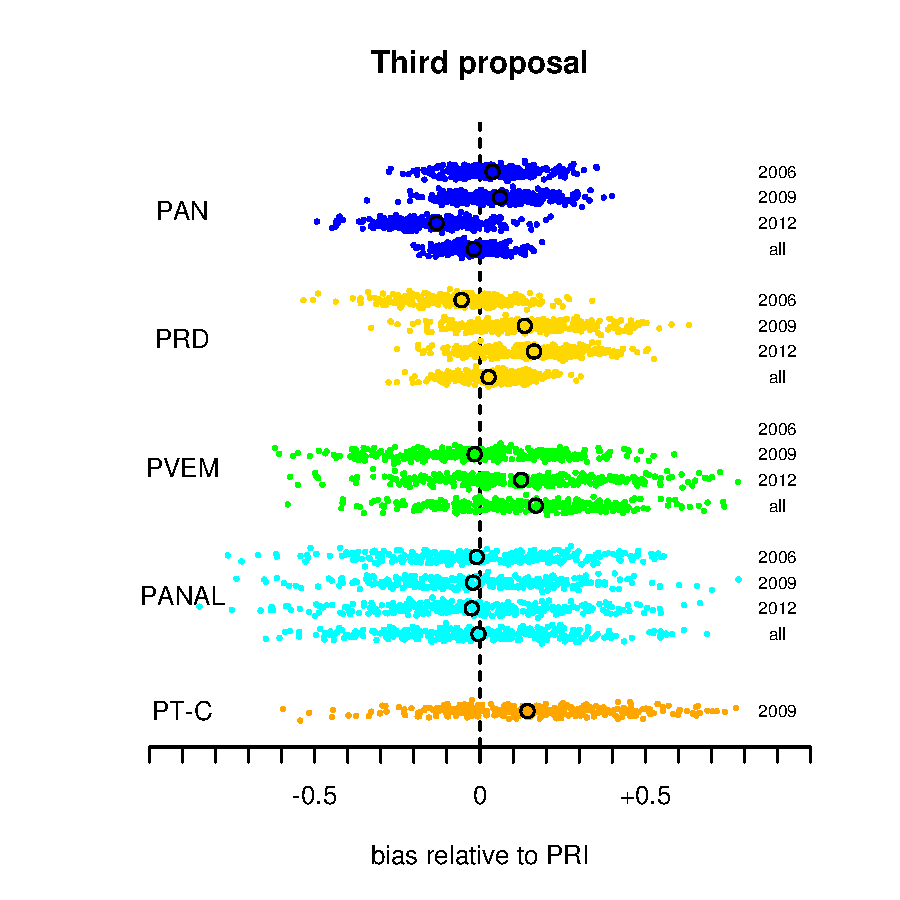
\includegraphics[width=5cm]{../../graphs/bias200612s3.pdf}
\end{tabular}
\end{center}
}
%%%%%%%%%%%%%%%%%%%%%%%%%%%%%%%%%%%%%%%%%%%%%%%%%%%%%%%%%%%%%%%%%%%%%%%%%%%%%%%%%%%%%%%%%%%% 
\frame {                      % SLIDE
    \frametitle{Results: responsiveness}
\begin{center}
   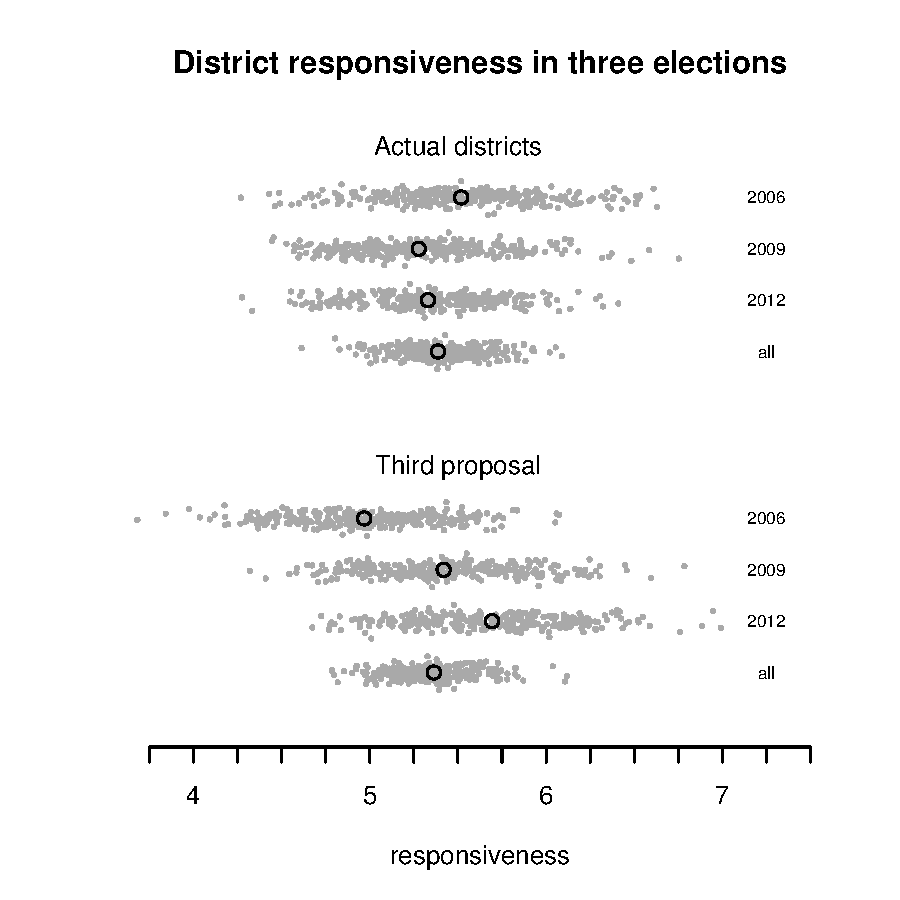
\includegraphics[width=6cm]{../../graphs/resp200612s0s3.pdf}
\end{center}
}

%%%%%%%%%%%%%%%%%%%%%%%%%%%%%%%%%%%%%%%%%%%%%%%%%%%%%%%%%%%%%%%%%%%%%%%%%%%%%%%%%%%%%%%%%%%%%%%%
\frame {                      % SLIDE
    \frametitle{Approach 2: seats--votes swing ratios (Niemi\&Fett 1986)}

\textbf{Swing ratio} is the \% change in seats associated with \\ a 1\% change in a party's national congressional vote 

\bigskip

Party with 10\% natl vote evenly spread v.\ concentrated in a region

\bigskip

Complication: who loses when party X wins 1\% nationwide? And where?

\bigskip

Further complication: two- v.\ multi-party systems

\bigskip

Linzer (2012): finite mixture model to simulate multiparty dynamics with compositional variable

}
%%%%%%%%%%%%%%%%%%%%%%%%%%%%%%%%%%%%%%%%%%%%%%%%%%%%%%%%%%%%%%%%%%%%%%%%%%%%%%%%%%%%%%%%%%%%%%%%
\frame {                      % SLIDE
    \frametitle{Mixture model}
\begin{itemize}
\item Combines the properties of two or more prob.\ density functions: can approximate any arbitrary distribution
\item Seek components (multivariate normals)  and weights of log-ratio votes shares
\end{itemize}

\begin{tabular}{cc}
   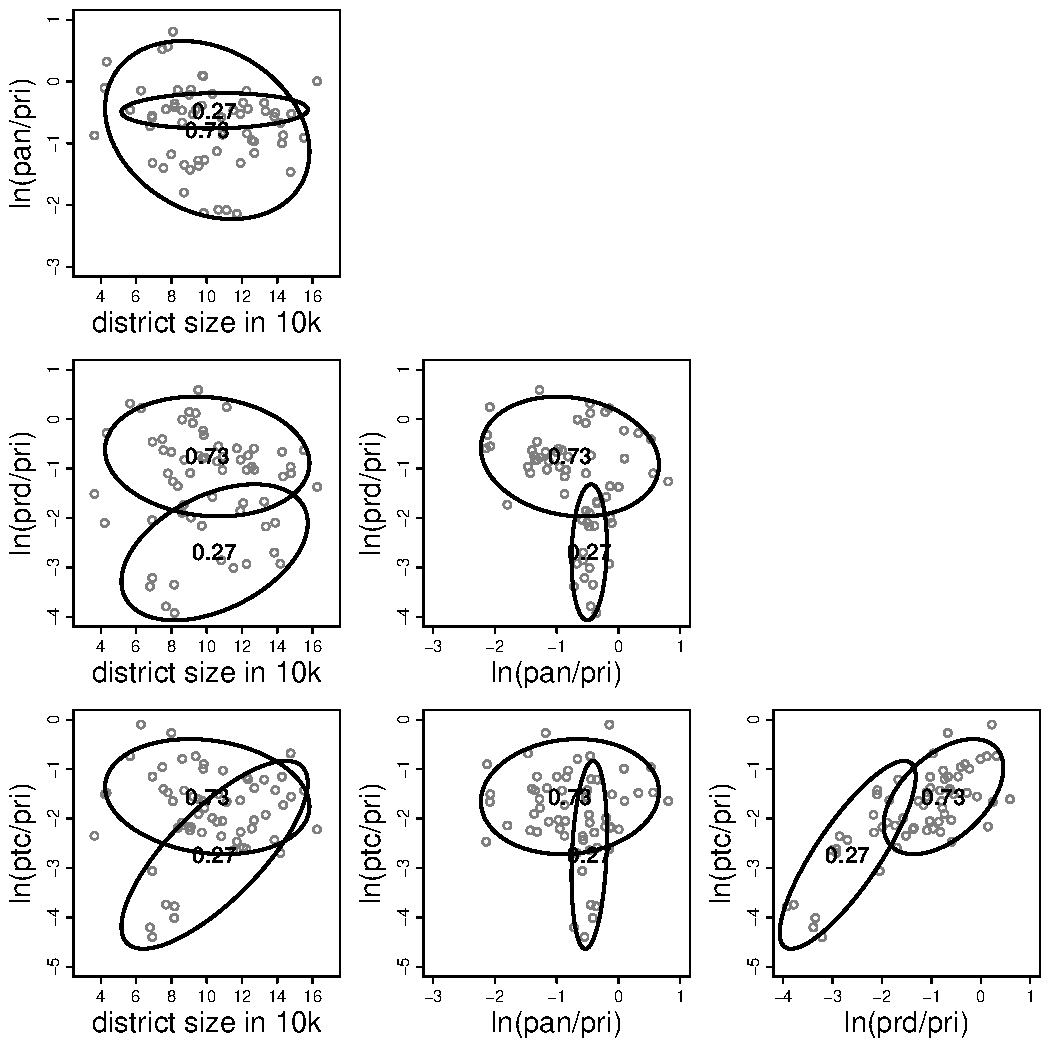
\includegraphics[width=4.95cm]{../../graphs/linzerLogVot2009-1.pdf} &
   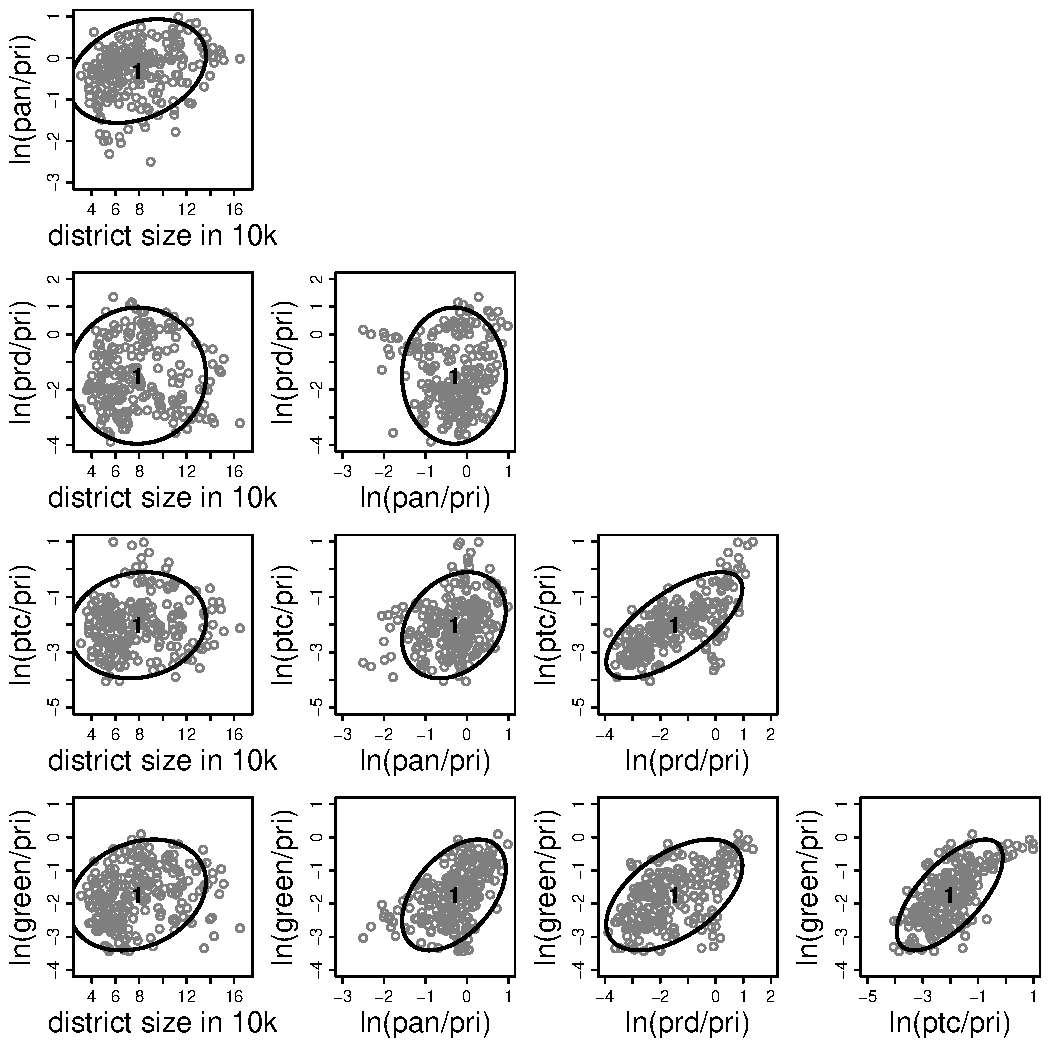
\includegraphics[width=4.95cm]{../../graphs/linzerLogVot2009-2.pdf}
\end{tabular}
 
}
%%%%%%%%%%%%%%%%%%%%%%%%%%%%%%%%%%%%%%%%%%%%%%%%%%%%%%%%%%%%%%%%%%%%%%%%%%%%%%%%%%%%%%%%%%%%%%%%
\frame {                      % SLIDE
    \frametitle{Fit: marginal densities}
\begin{center}
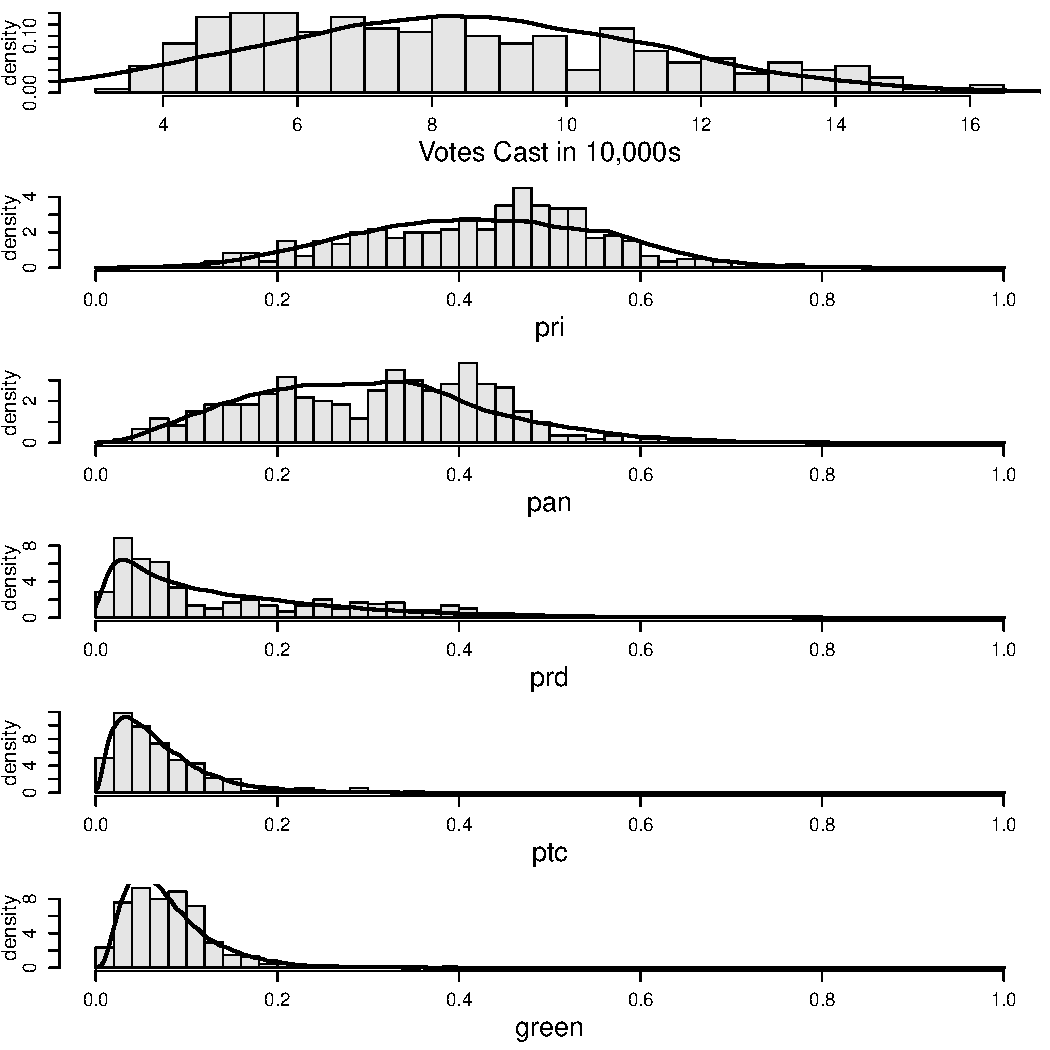
\includegraphics[width=5cm]{../../graphs/linzerMarg2009.pdf}
\end{center}
}
%%%%%%%%%%%%%%%%%%%%%%%%%%%%%%%%%%%%%%%%%%%%%%%%%%%%%%%%%%%%%%%%%%%%%%%%%%%%%%%%%%%%%%%%%%%%%%%%
\frame {                      % SLIDE
    \frametitle{Trade-offs: 1,000 simulated 2009 elections}

\begin{center}
\begin{tabular}{cc}
    Vote shares & Seat shares \\
    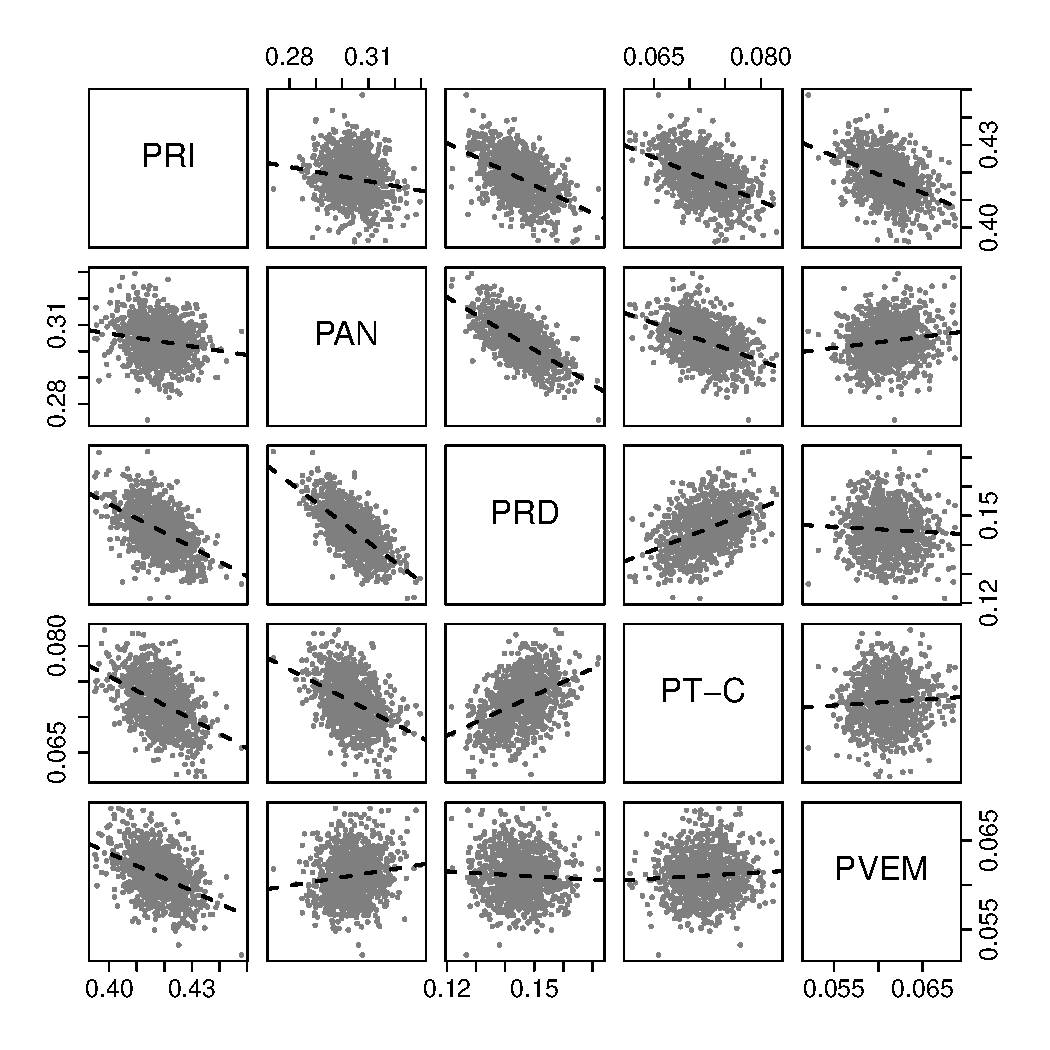
\includegraphics[width=.475\columnwidth]{../../graphs/linzerVoteSims2009.pdf} &
    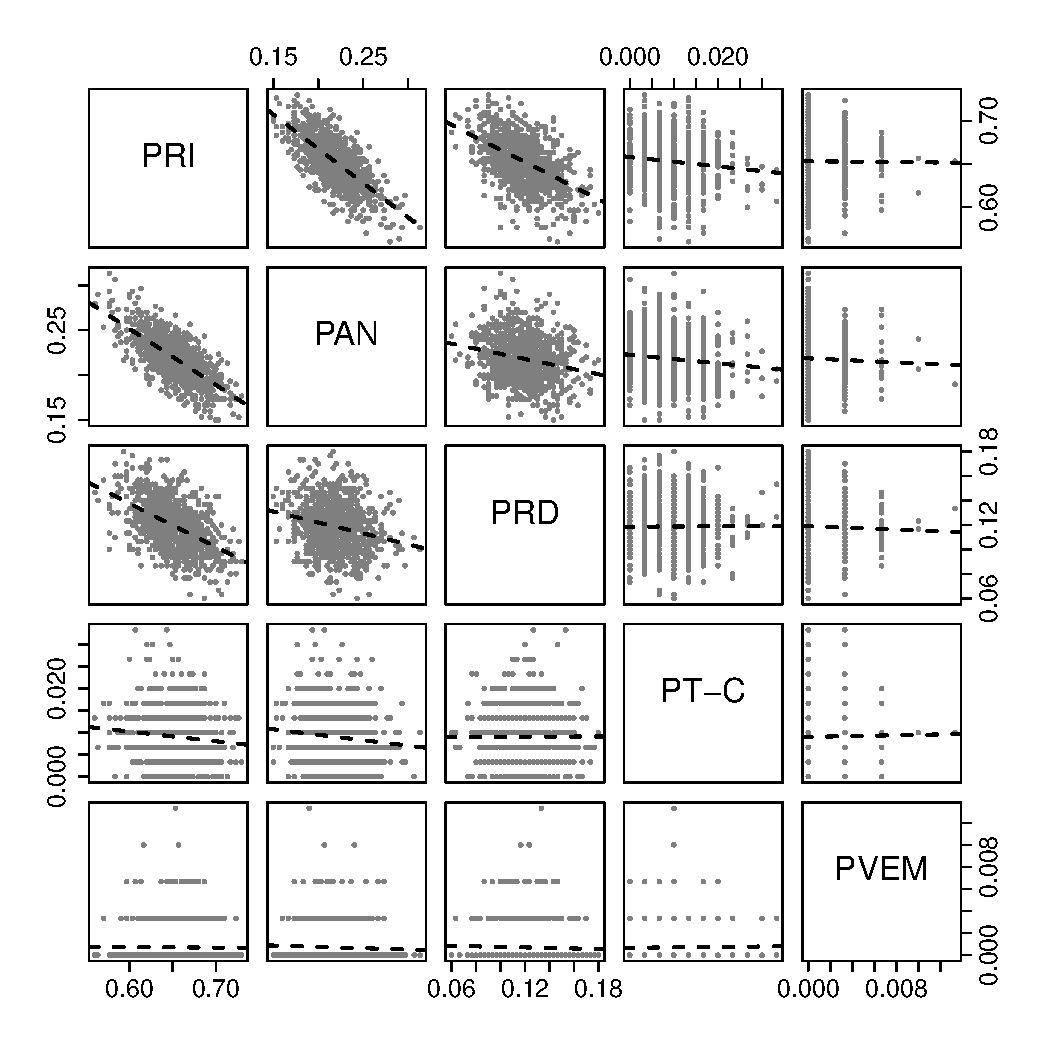
\includegraphics[width=.475\columnwidth]{../../graphs/linzerSeatSims2009.pdf} 
  \end{tabular}
\end{center}

}
%%%%%%%%%%%%%%%%%%%%%%%%%%%%%%%%%%%%%%%%%%%%%%%%%%%%%%%%%%%%%%%%%%%%%%%%%%%%%%%%%%%%%%%%%%%%%%%%
\frame {                      % SLIDE
    \frametitle{Use swing ratios to compare two maps}

\begin{enumerate}
\item Simulate 5k 2009 elections with status quo map for each party
\item Repeat using abandoned map
\item Pool simulations together and regress
\item Coefficient $\beta_3$ measures and tests change in \\ party's swing ratio \emph{due to redistricting} 
\end{enumerate}

\bigskip

$S = \beta_0 + \beta_1 V + \beta_2 dis2015 + \beta_3 V \times dis2015 + \texttt{error}$

}
%%%%%%%%%%%%%%%%%%%%%%%%%%%%%%%%%%%%%%%%%%%%%%%%%%%%%%%%%%%%%%%%%%%%%%%%%%%%%%%%%%%%%%%%%%%%%%%%
\frame {                      % SLIDE
    \frametitle{Results}
\begin{center}

% \begin{tabular}{lrrrrrr}
%                    & \multicolumn{2}{c}{PAN}   & \multicolumn{2}{c}{PRI}   & \multicolumn{2}{c}{Left}   \\
%                    & $\hat{\beta}$ & $p$-val. & $\hat{\beta}$ & $p$-val. & $\hat{\beta}$ & $p$-val.  \\ \hline
% ~~\textbf{2006 election} \\
% $V$                &     1.94 & $<.001$&   2.27 &$<.001$&   1.91 &$<.001$\\
% $V \times$ dis2015 &     \alert<2>{+.45} & $<.001$&  $-.01$&  .809 &  $-.04$&  .183 \\
% ~~\textbf{2009 election} \\
% $V$                &     1.95 & $<.001$&   2.27 &$<.001$&   1.67 &$<.001$\\
% $V \times$ dis2015 &    $-.13$&   .003 &   +.04 &  .354 &  $-.02$&  .623 \\
% ~~\textbf{2012 election} \\
% $V$                &     2.24 &$<.001$ &   3.99 &$<.001$&   2.39 &$<.001$\\
% $V \times$ dis2015 &     +.02 &   .604 &   +.03 &  .720 &  $-.06$&  .103 \\ \hline
% \end{tabular}

\begin{tabular}{lr@{}lr@{}lr@{}l}
                   & \multicolumn{2}{c}{PAN}   & \multicolumn{2}{c}{PRI}   & \multicolumn{2}{c}{Left} \\ \hline
~~\textbf{2006 election} \\
$V$                &     1.94 & $^{***}$&   2.27 & $^{***}$&   1.91 & $^{***}$\\
$V \times$ dis2015 &     \alert{+.45} & $^{***}$&  $-.01$&        &  $-.04$&        \\
~~\textbf{2009 election} \\
$V$                &     1.95 & $^{***}$&   2.27 & $^{***}$&   1.67 & $^{***}$\\
$V \times$ dis2015 &    \alert{$-.13$}& $^{***}$&   +.04 &        &  $-.02$&        \\
~~\textbf{2012 election} \\
$V$                &     2.24 & $^{***}$&   3.99 & $^{***}$&   2.39 & $^{***}$\\
$V \times$ dis2015 &     +.02 &        &   +.03 &       &  \alert{$-.06$} &  $^{*}$ \\ \hline
\multicolumn{7}{l}{\footnotesize{$^{***} <.01$, $^{*} <.1$}}
\end{tabular}

\end{center}
}
%%%%%%%%%%%%%%%%%%%%%%%%%%%%%%%%%%%%%%%%%%%%%%%%%%%%%%%%%%%%%%%%%%%%%%%%%%%%%%%%%%%%%%%%%%%%%%%%

\frame {                      % SLIDE

    \frametitle{Findings, next steps}

Preliminary analysis reveals that:

\begin{enumerate}

\item Malapportionent is substantial

\item Yet no evidence of systematic party bias

\item But \textbf{huge} large-party bonus (PRI is small in few states)

\item And boundary changes affect more PAN than PRD, and especially than PRI

\item Study inter-election volatility? 

\item Study residuals and relation to malapp.? turnout diff.? geography of support?

\end{enumerate}

\pause

\bigskip

\center{\textbf{\Large{Thank you!}}}

}
\end{document}

%%%%%%%%%%%%%%%%%%%%%%%%%%%%%%%%%%%%%%%%%%%%%%%%%%%%%%%%%%%%%%%%%%%%%%%%%%%%%%%%%%%%%%%%%%%%
\frame {                      % SLIDE
    \frametitle{Tit}
}
